%SURPRISE: There is more than one type of insulator
\begin{frame}{Topological Band Insulators}
\vskip-1.5cm
Topological bands discovered in Integer Quantum Hall Effect (IQHE) (1984)
\begin{columns}[T]
\begin{column}[T]{0.65\textwidth}
\bi
\item Bulk conductance drops to 0
\item Integer filling of Landau levels
%There is some notion of integer charge per site that remains, but magnetic field (vector potential) messes with naive translational invariance
\item Robust chiral edge modes
\item Quantized Hall conductivity $\sigma_H = n\frac{e^2}{\hbar}$
\item No longer an atomic insulator
\item<2-> Topological invariant Chern number (a.k.a. TKNN)
%Chern number is a total curvature integrated over the Brillouin zone
\ei
\end{column}
\begin{column}[T]{0.35\textwidth}
\only<1, 3>{
\begin{figure}
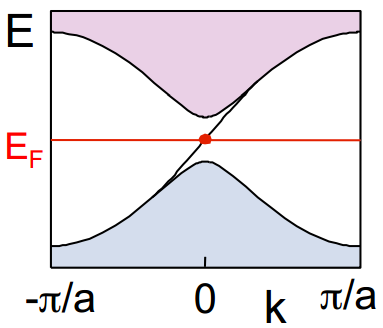
\includegraphics[width=\linewidth]{diagrams/chiral_edge.png}
\caption{Chiral Edge \footnotemark}
\end{figure} 
}
\only<2>{
\begin{figure}
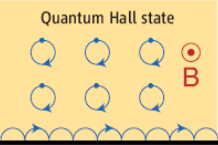
\includegraphics[width=\linewidth]{diagrams/bernevig2.png}
\caption{Chiral Edge}
\end{figure} 
}
\end{column}
\end{columns}

\only<3->{
$$
n^{\alpha} = \frac{i}{2\pi} \int_{B.Z.} d^2\kk \bra{\partial_{\kk_x} u^{\alpha}_{\kk}}  \ket{\partial_{\kk_y}u^{\alpha}_{\kk}}-\bra{\partial_{\kk_y} u^{\alpha}_{\kk}}  \ket{\partial_{\kk_x}u^{\alpha}_{\kk}}
$$
}
\footnotetext[1]{
\citep{Hasan2010-fq}} %\footfullcite{HasanKane}?
\end{frame}